\section{I/O level Refinement}
\label{sec:component_diagrams-ioLevel}

The tutorial in the previous section demonstrates how to perform abstract modelling and refinement using the CODA component diagram tools. This section illustrates how a refinement can be introduced which models the hardware I/O level behaviour. The model uses a synchronised state-machine, which allows a sequence of clock synchronised I/O events to be performed in order to achieve an abstract data transmission.

 \begin{figure}[!htbp]
  \centering
  \ifplastex
  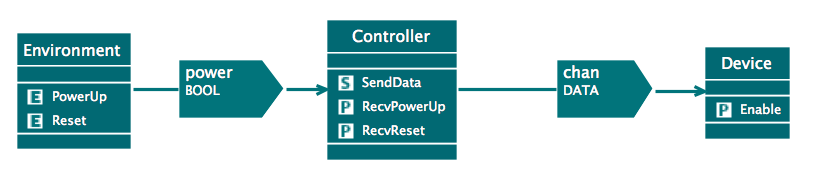
\includegraphics[width=1024]{figures/image53.png}
  \else
  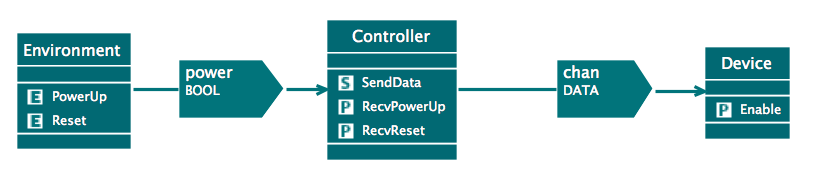
\includegraphics[width=1\textwidth]{figures/image53.png}
  \fi
  \caption{Abstract Model of a Controller Sending an Enable Message to a Device}
  \label{fig:AbstractModelOfAControllerSendingAnEnableMessageToADevice}
\end{figure} 

In the abstract model, shown in Figure \ref{fig:AbstractModelOfAControllerSendingAnEnableMessageToADevice}, a Controller component sends data to enable a Device component. This is modelled as a port-send belonging to a self-wake operation SendData, a connector chan and a port-wake operation Enable. The self-wake is scheduled by the RecvPowerUp operation, so that its timing represents the completion of an envisaged concrete operation which takes time to complete.

 \begin{figure}[!htbp]
  \centering
  \ifplastex
  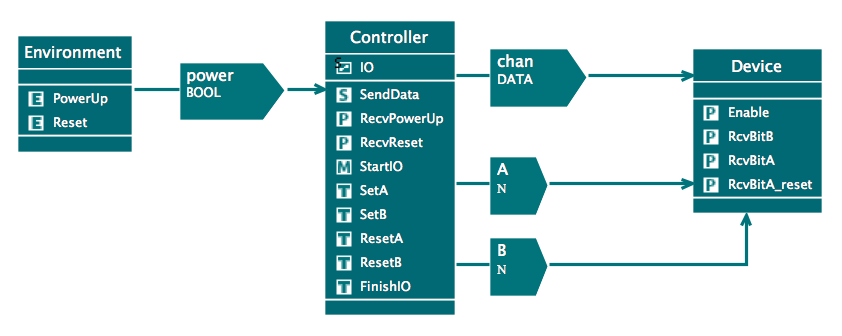
\includegraphics[width=1024]{figures/image54.png}
  \else
  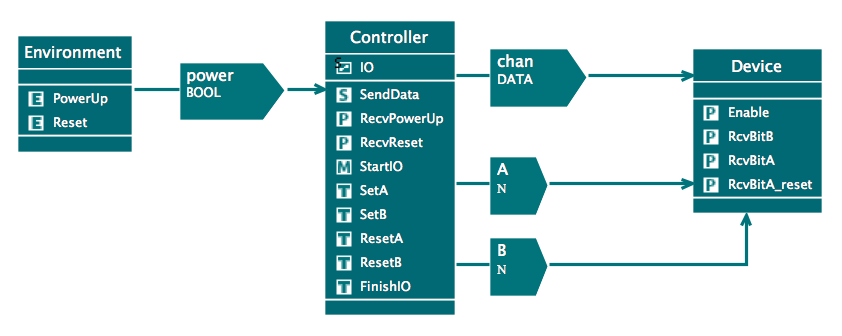
\includegraphics[width=1\textwidth]{figures/image54.png}
  \fi
  \caption{Refined Model : Controller Sending a Bit Level Signal to a Device}
  \label{fig:RefinedModelControllerSendingABitLevelSignalToADevice}
\end{figure} 

In the refined model, shown in Figure \ref{fig:RefinedModelControllerSendingABitLevelSignalToADevice}, the concrete data transmission operations are introduced. In this example, two connectors are used, A for the data bit stream and B for a data ready semaphore. Operations, SetA, SetB, ResetA and ResetB send 1 and 0 on these connector channels respectively. In order to ensure these operations are invoked in the desired iterative sequence, a synchronised state-machine IO is attached to the Controller component. 

 \begin{figure}[!htbp]
  \centering
  \ifplastex
  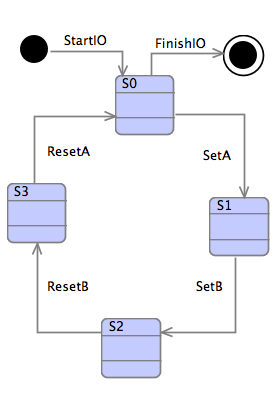
\includegraphics[width=1024]{figures/image55.png}
  \else
  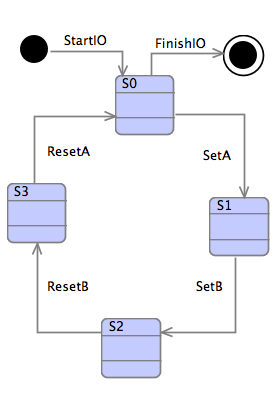
\includegraphics[width=1\textwidth]{figures/image55.png}
  \fi
  \caption{Refined Model : I/O Level State-machine}
  \label{RefinedModelIOLevelStatemachine}
\end{figure} 

The transitions of this state-machine, Figure \ref{RefinedModelIOLevelStatemachine}, are linked to the same events as the component operations that send the data bits. Hence these operations are constrained to execute in the iterative sequence defined by the state-machine. Furthermore, because this is a synchronised state-machine, it is forced to fire exactly one transition on each clock cycle while it is enabled. The state-machine becomes enabled when the initial transition is taken and this is linked to a method operation of the Controller component that is called by the RecvPowerUp operation. Guards and Actions in the bit sending operations allow the state-machine to complete 16 cyclic sequences before taking the FinishIO transition that disables the state-machine. The data sent by the operation SendData was calculated to be received by operation Enable at the same clock cycle as the last bit is received on connector A representing the end of the bit level transmission.
In this refinement the abstract data connector and associated operation behaviour have been retained although they are now redundant because they are replaced by the I/O level connector behaviour. It would be tempting to remove the abstract data connector and prove that the I/O level is a refinement of it. However, it may be useful to retain the abstract data connector for later generation of temporal assertions in generated output such as VHDL.

%%% Local Variables:
%%% mode: latex
%%% TeX-master: "component_diagrams-user_manual"
%%% End:
